% !TeX root=../main.tex
\chapter{نتایج}
%\thispagestyle{empty} 
\label{chap:results}
\section{مقدمه} 
در فصل‌های قبل درباره معماری میکروسرویس و درستی‌سنجی نرم‌افزار صحبت کردیم. سپس روشی مبتنی بر طراحی بر اساس قرارداد معرفی کردیم. در این روش روی درستی‌سنجی ارتباط بین میکروسرویس‌ها تمرکز کردیم و به طور خاص گفتیم که در روش ما می‌توان روی ترتیب اجرای فراخوانی‌های از راه دور شرط نوشت. در این فصل،‌ با استفاده از روشمان و کتابخانه‌ای که توسعه دادیم به درستی‌سنجی یک برنامه با معماری میکروسرویس می‌پردازیم و نشان می‌دهیم که چگونه در آن اشکالاتی را پیدا کردیم. در نهایت سربار روشمان را روی کارایی برنامه بررسی می‌کنیم و نشان می‌دهیم که روش ما سربار بسیار کمی خواهد داشت.

\section{درستی‌سنجی برنامه فروشگاه آنلاین}
برای ارزیابی روشمان در یک برنامه واقعی، پروژه
\lr{microservices-demo} \cite{microservicesDemo}
شرکت گوگل را درستی‌سنجی کردیم. این پروژه یک فروشگاه آنلاین است که از چندین میکروسرویس تشکیل شده است. معماری این برنامه در تصویر
\ref{fig:arch}
و توضیحات هر میکروسرویس در جدول
\ref{tab:microservices}
آمده است.

\begin{figure}[ht]
\centerline{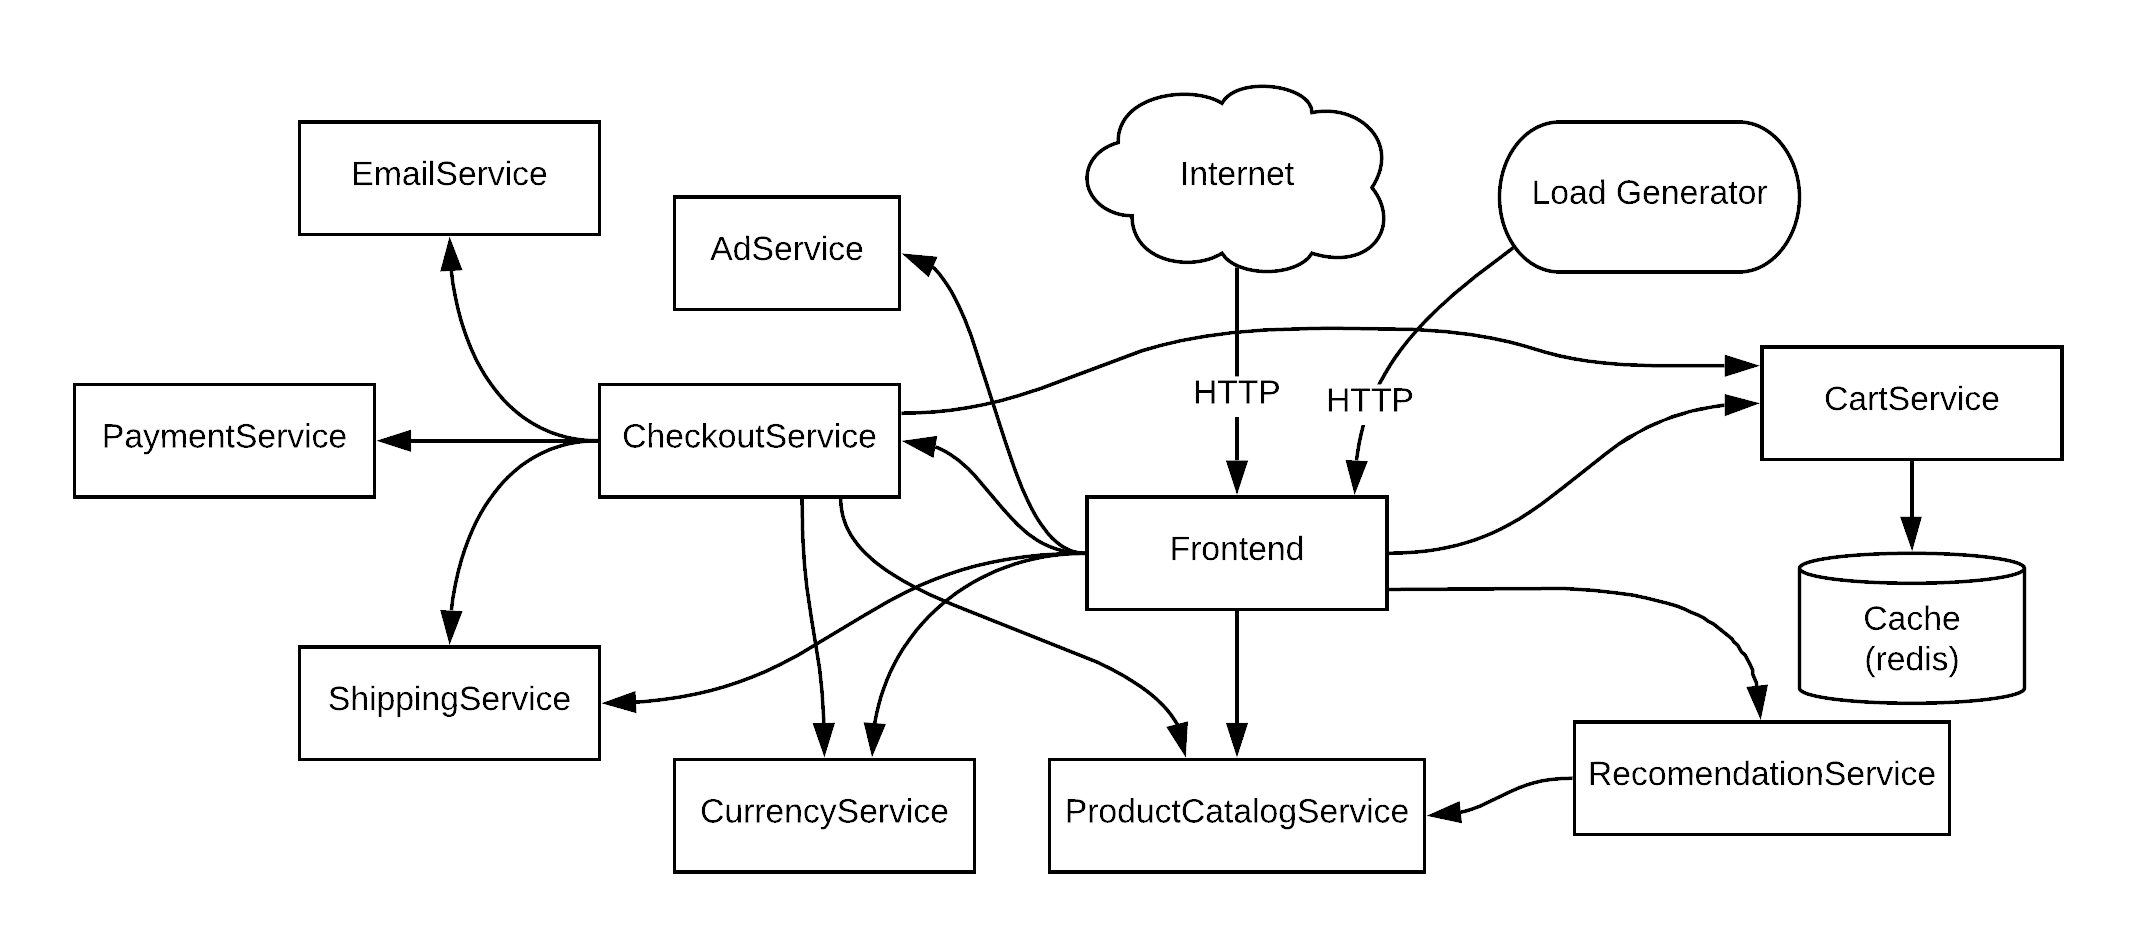
\includegraphics[width=15cm]{architecture-diagram.png}}
\caption{معماری برنامه فروشگاه آنلاین}
\label{fig:arch}
\end{figure}

\begin{table}
    \caption{توضیح میکرویس‌های فروشگاه آنلاین}
    \label{tab:microservices}
    \centering
    \begin{tabular}{|l|l|l|}
    \hline
        سرویس & زبان برنامه‌نویسی & توضیحات \\ \hline
        Frontend & Go & رابط کاربری \\ \hline
        CartService & C\# & ذخیره سبد خرید \\ \hline
        ProductCatalogService	 & Go & اطلاعات کالاها \\ \hline
        CurrencyService & Node.js & تبدیل ارز‌های مختلف \\ \hline
        PaymentService & Node.js & پرداخت \\ \hline
        ShippingService & Go & تعیین هزینه ارسال و ارسال کالا \\ \hline
        EmailService & Python & ارسال ایمیل \\ \hline
        CheckoutService & Go & ثبت سفارش \\ \hline
        RecommendationService & Python & پیشنهاد کالا \\ \hline
        AdService & Java & ارائه تبلیغات \\ \hline
        LoadGenerator & Python/Locust & ایجاد ترافیک \\ \hline
    \end{tabular}
\end{table}
ما درستی‌سنجی را روی میکروسرویس‌های 
\lr{CheckoutService}،
\lr{ProductCatalogService}
و
\lr{ShippingService}
که با زبان
Go
نوشته شده بودند انجام دادیم
\cite{forkedMicroservicesDemo}
و در نهایت توانستیم سه اشکال در این برنامه پیدا کنیم.

\subsection{
سرویس CheckoutService
}

\singlespacing
\begin{figure}
	\begin{LTR}
		\lstinputlisting[language=protobuf2, breaklines=true, basicstyle=\ttfamily\footnotesize, caption={سرویس CheckoutService}, label={code:CheckoutProto}]{checkout.proto}
	\end{LTR}
\end{figure}
\doublespacing

این سرویس وظیفه ثبت سفارش را بر عهده دارد و توصیف رابط آن در برنامه
\ref{code:CheckoutProto}
آمده است. شرط‌های زیر را در یک قرارداد برای فرخوانی
\lr{\texttt{PlaceOrder}}
تعریف کردیم.

پیش‌شرط‌ها:
\begin{enumerate}
\item
ایمیل کاربر معتبر باشد.
\item
کارت اعتباری کاربر معتبر باشد.
\item
احراز هویت کاربر تایید شده باشد.
\end{enumerate}

پس‌شرط‌ها:
\begin{enumerate}
\item
در صورت موفقیت‌آمیز بودن خروجی تابع
\lr{\texttt{PlaceOrder}}
، باید تابع
\lr{\texttt{Charge}}
در سرویس
\lr{\texttt{PaymentService}}
با موفقیت فراخوانی شده باشد.
\item
تابع
\lr{\texttt{Charge}}
باید قبل از تابع
\lr{\texttt{ShipOrder}}
فراخوانی شده باشد.
\end{enumerate}

پیش‌شرط‌های ۱ و ۲ سبب پیدا شدن دو اشکال در برنامه شدند. چرا که بررسی درستی این مقادیر در رابط کاربری صورت می‌گرفت و در صورت فراخوانی مستقیم
\lr{API}ها
می‌توان داده نادرست به آن‌ها داد و برنامه نیز آن‌ها را قبول می‌کند.


\subsection{
سرویس ShippingService
}

\singlespacing
\begin{figure}
	\begin{LTR}
		\lstinputlisting[language=protobuf2, breaklines=true, basicstyle=\ttfamily\footnotesize, caption={سرویس ShippingService}, label={code:ShippingProto}]{shipping.proto}
	\end{LTR}
\end{figure}
\doublespacing

این سرویس وظیفه ارسال سفارش را بر عهده دارد و توصیف رابط آن در برنامه
\ref{code:ShippingProto}
آمده است. شرط‌های زیر را در یک قرارداد برای فرخوانی
\lr{\texttt{ShipOrder}}
تعریف کردیم.

پیش‌شرط‌ها:
\begin{enumerate}
\item
تعداد کالای از یک نوع باید نامنفی باشد.
\end{enumerate}

پس‌شرط‌ها:
\begin{enumerate}
\item
در صورت موفقیت‌آمیز بودن خروجی تابع
\lr{\texttt{ShipOrder}}
مقدار
\lr{\texttt{TrackingId}}
در خروجی نباید خالی باشد.
\end{enumerate}

پیش‌شرط ۱ باعث پیدا شدن یک اشکال دیگر در برنامه شد، چرا بررسی این شرط در برنامه به‌هیچ وجه انجام نمی‌شد.

\subsection{
سرویس ProductCatalogService
}

این سرویس وظیفه برگرداندن اطلاعات یک کالا را دارد و توصیف رابط در برنامه
\ref{code:ProductProto}
آمده است. شرط‌های زیر را در یک قرارداد برای فراخوانی
\lr{\texttt{GetProduct}}
تعریف کردیم.
پس‌شرط‌ها:
\begin{enumerate}
\item
مقدار ID در درخواست باید با مقدار ID در کالای برگردانده‌شده برابر باشد.
\end{enumerate}

\singlespacing
\begin{figure}
	\begin{LTR}
		\lstinputlisting[language=protobuf2, breaklines=true, basicstyle=\ttfamily\footnotesize, caption={سرویس ProductCatalogService}, label={code:ProductProto}]{productcatalog.proto}
	\end{LTR}
\end{figure}
\doublespacing


\section{سربار کارایی}
ما برای بررسی میزان سرباری که کتابخانه‌مان ایجاد می‌کند، ترافیک مشابهی در دو حالت روی برنامه ایجاد کردیم. اول در حالتی که بررسی قراردادها انجام شود، و دیگر بدون اینکه قراردادی تعریف شود. برای ایجاد ترافیک، رفتار تعداد کاربران همزمان را روی این برنامه شبیه‌سازی کردیم و سپس میانه زمان پاسخگویی به یکی از فراخوانی‌ها را اندازه‌گیری کردیم. خروجی این آزمایش در تصویر
\ref{fig:performance}
آمده است. همان‌طور که مشخص است، سربار زمانی ایجاد کاملا ناچیز است. همینطور در آزمایش‌های ما سربار حافظه نیز مقدار بسیار کوچکی بود.

\begin{figure}[t]
\centering
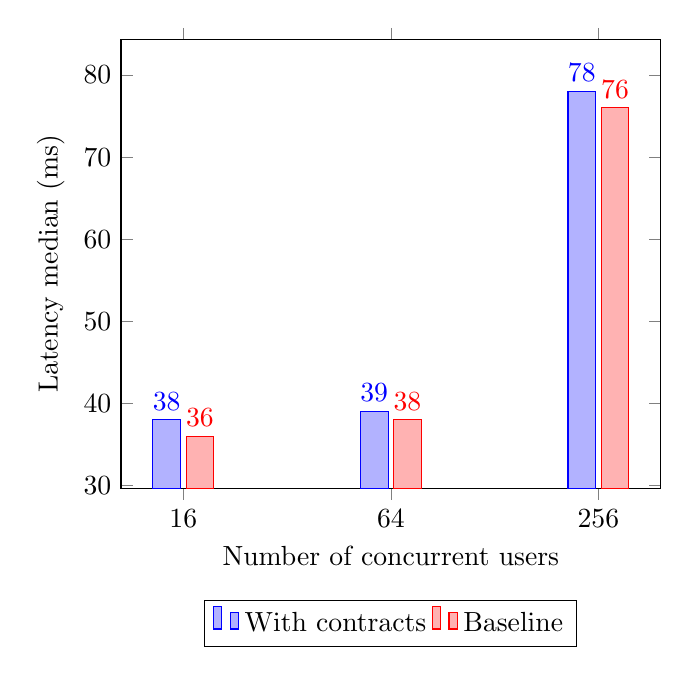
\begin{tikzpicture}
\begin{axis}[
    ybar,
    enlargelimits=0.15,
    legend style={at={(0.5,-0.25)},
      anchor=north,legend columns=-1},
    ylabel={Latency median (ms)},
    xlabel={Number of concurrent users},
    symbolic x coords={16, 64, 256},
    xtick=data,
    nodes near coords,
    nodes near coords align={vertical},
    ]
\addplot 
	coordinates {(16, 38) (64, 39) (256, 78)};
\addplot 
	coordinates {(16, 36) (64, 38) (256, 76)};
\legend{With contracts, Baseline}
\end{axis}
\end{tikzpicture}
\caption{مقایسه زمان پاسخگویی}
\label{fig:performance}
\end{figure}
